\documentclass[12pt]{article}
\usepackage[breaklinks=true]{hyperref}
\usepackage[margin=0.75in]{geometry}

\usepackage{graphicx}
\usepackage{color}
\usepackage{amsmath}

\definecolor{pblue}{rgb}{0.13,0.13,1}
\definecolor{pgreen}{rgb}{0,0.5,0}
\definecolor{pred}{rgb}{0.9,0,0}
\definecolor{pgrey}{rgb}{0.46,0.45,0.48}

\usepackage{listings}
\lstset{language=Java,
  showspaces=false,
  showtabs=false,
  tabsize=2,
  breaklines=true,
  showstringspaces=false,
  breakatwhitespace=true,
  numbers=left,
  commentstyle=\color{pgreen},
  keywordstyle=\color{pblue},
  stringstyle=\color{pred},
  basicstyle=\ttfamily,
  frame=single,
  moredelim=[il][\textcolor{pgrey}]{$$},
  moredelim=[is][\textcolor{pgrey}]{\%\%}{\%\%}
}

\title{GUIs in Java}
\author{
	Melvyn Ian Drag
}
\date{\today}


\begin{document}
\maketitle

\begin{abstract}
So far all of our projects have only done input/output on the command line.
Today we will add a GUI to a project.
\end{abstract}

\section{Introduction}
A GUI is a \textbf{Graphical User Interface}. The term refers to a program with
a pretty graphical front end that features things like buttons and sliders, will
perhaps show images and text in beautiful ways, and more. So far we've only done
commandline-driven programs, but you a probably more familiar with GUIs in the
form of various desktop applications. People who use Linux, BSD, and ( to a
lesser extent ) Macs are often comfortable with and happy to use command line
programs - the rest of the world, as a generalization, wants a GUI.

\section{Goal of the Night}
Tonight's class is something of a guided research project. We'll start with a
simple bit of code and then add some features to it.
\section{How to Make a GUI}
Two popular java libraries for making GUIs are \textit{swing} and \textit{awt}.
So far as I can tell, \textit{swing} is widely used and \textit{awt} is
considered old and only really used for teaching because it is very simple.
That's probably an unfair generalization, but that's what sticks in my memory
after a few months of reading about Java.

\subsection{A question!}
In our code today we will be importing stuff from both \textit{awt} and
\textit{swing}.

\begin{lstlisting}
import javax.swing.JFrame;
import javax.swing.JButton;
import javax.swing.JOptionPane;
import javax.swing.SwingUtilities;
import java.awt.event.ActionListener;
import java.awt.event.ActionEvent;
\end{lstlisting}

The \textit{ActionEvent} and \textit{ActionListener} are both from \textit{awt},
and these are the tools we use to program what our code does when a button is
clicked. Why are we mixing libraries here? Does \textit{swing} not have it's own
dedicated action handlers? This code we're using today I got randomly off the
internet on some Java blog.

See:
\textbf{Insert link here, when found, can't remember where I got the code and
I'm offline right now}

\section{Extra Credit Today}

\subsection{Objective}

\begin{figure}[h]
  \centering
    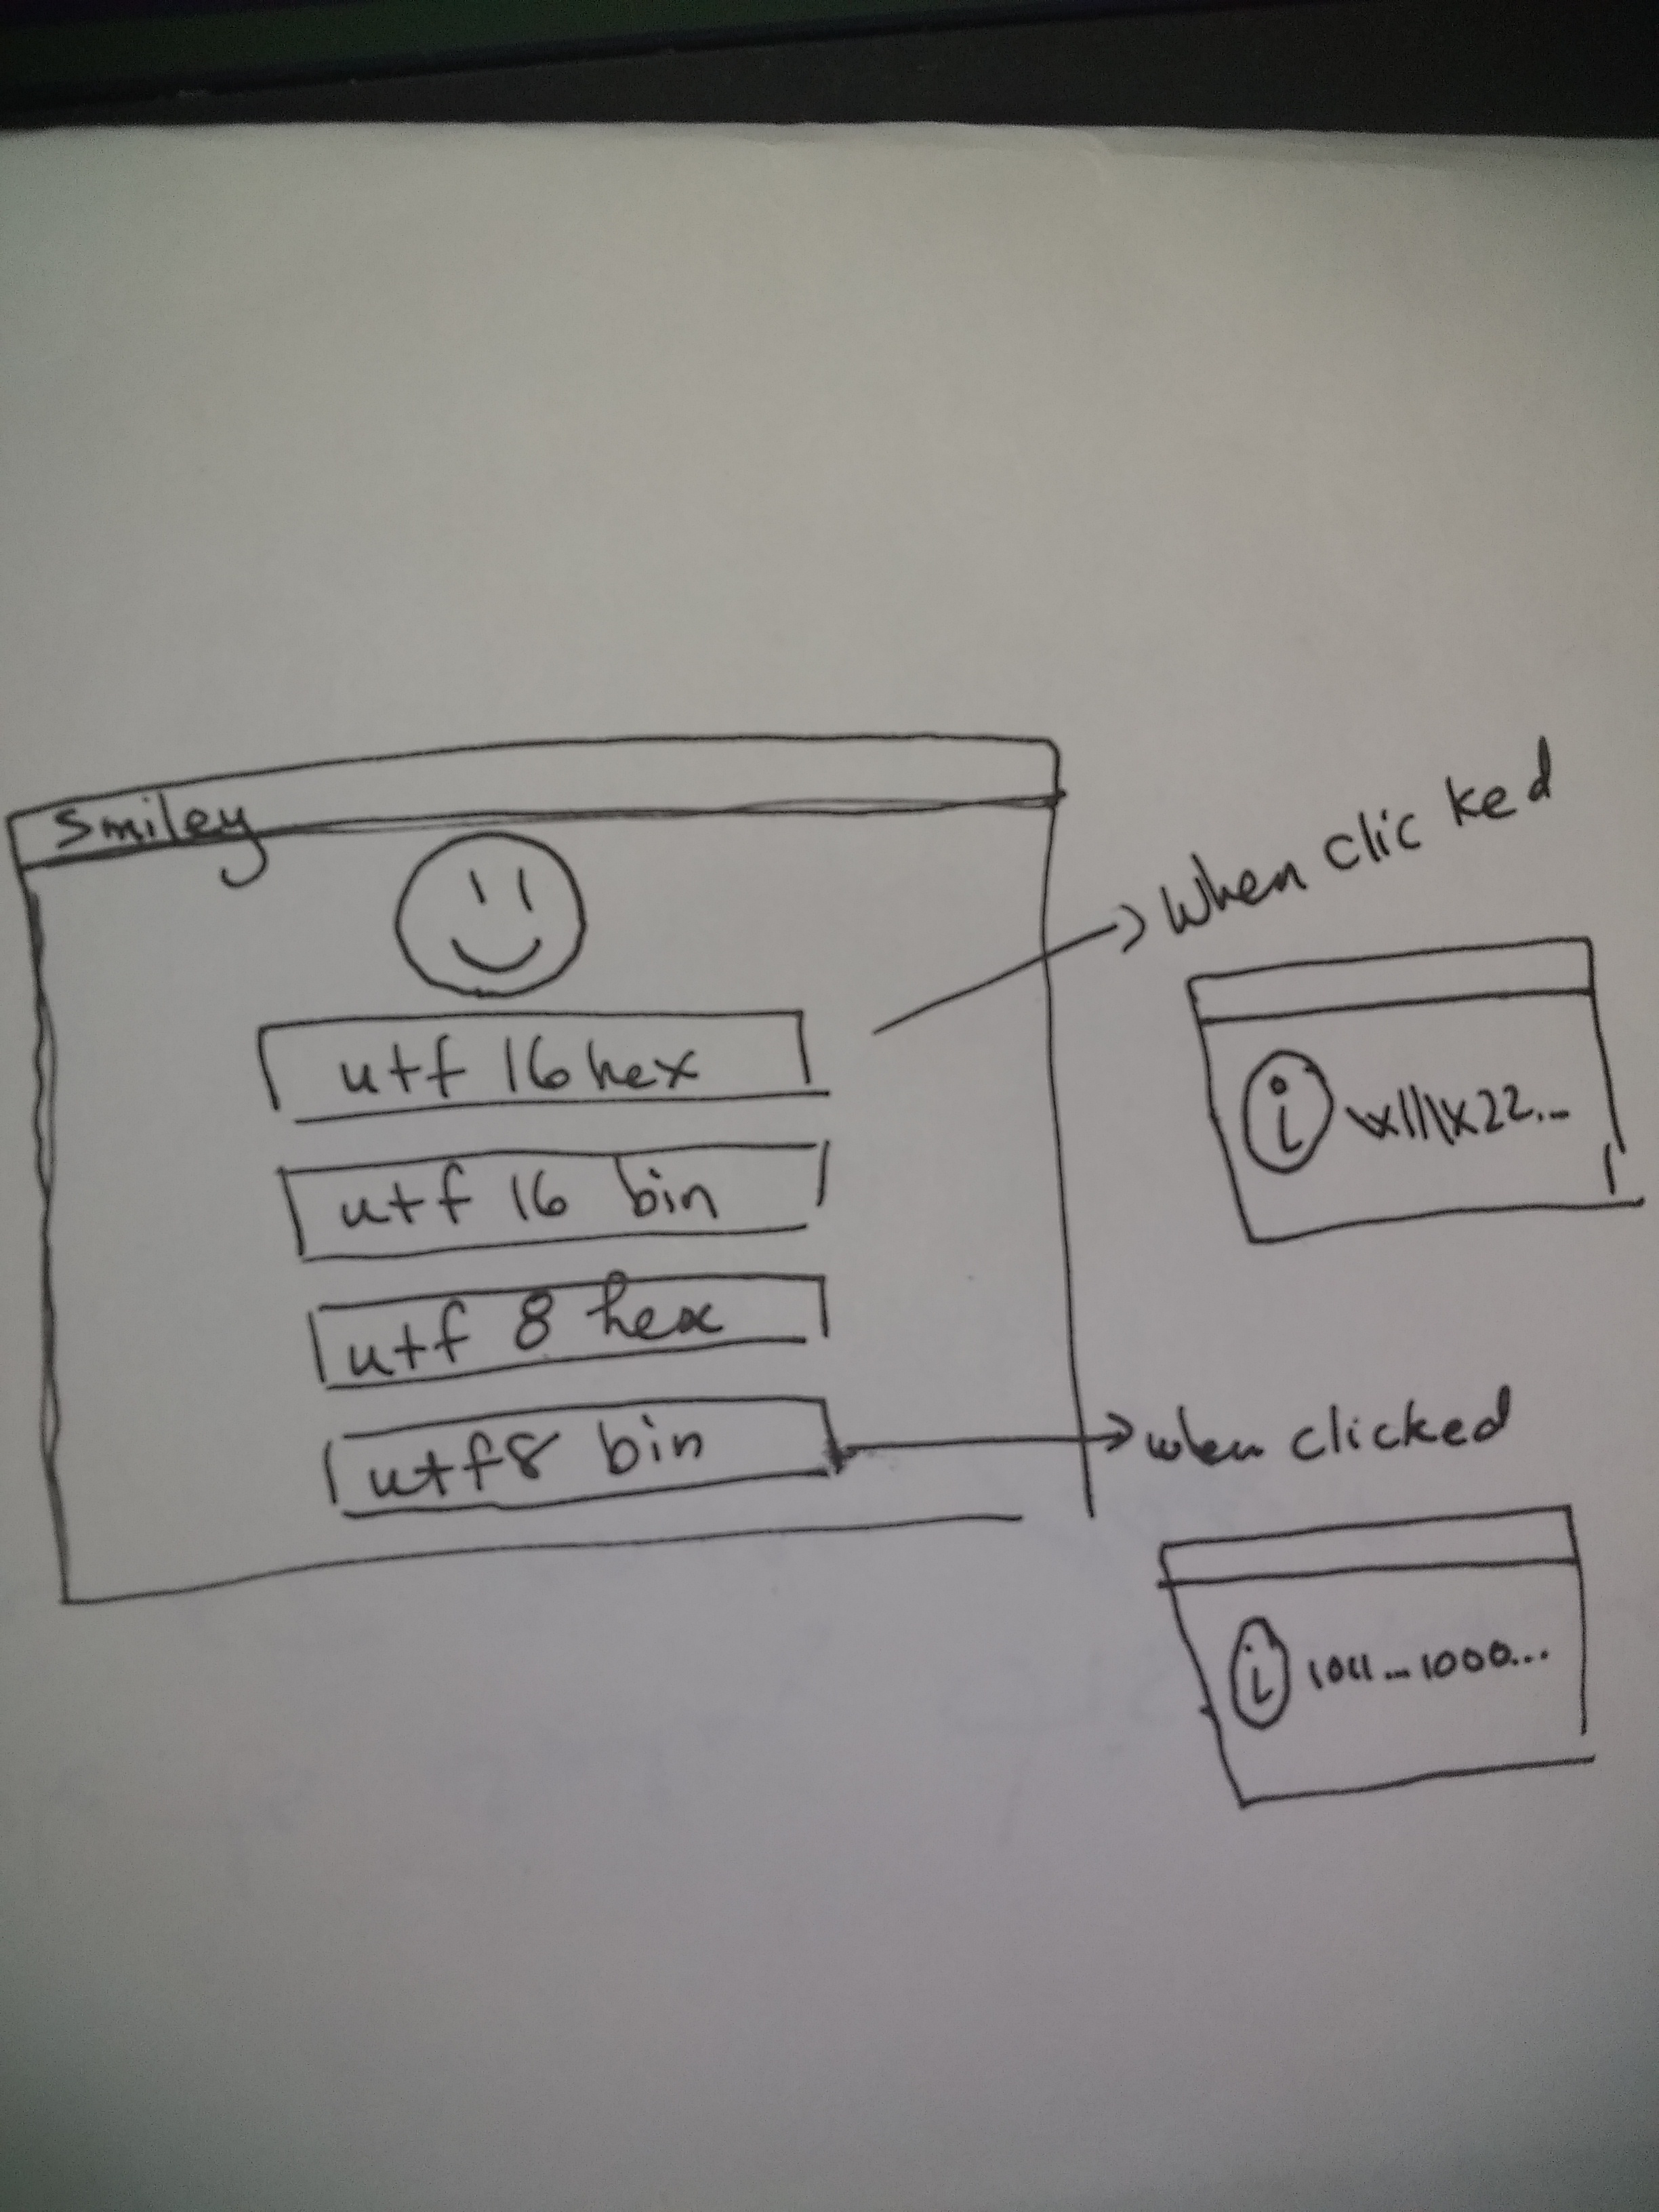
\includegraphics[width=0.9\textwidth]{Images/objective.jpg}
  \caption{Your goal for today.}
  \label{objective}
\end{figure}

I want you to create little application has 4 buttons. When clicked, 1 of them will print out the utf16 hex
representation of an emoji. The other will print the utf16 binary
representation. The other will print the utf8 hex. The last the utf8 binary. 

As you can see by the figure \ref{objective} this is just a little thing I
dreamt up and scribbled on the back of a piece of paper. But I've played with
the ideas involved and it is a doable assignment if you know a little bit of
Java!

Also, look at \ref{templateresult}. I've given you code that creates this
program. The code is very short and sweet, and does what we need! It has a
couple of buttons that, when clicked, throw up a little window with a string in
it. We just need to figure out what strings we want to show. Let's do that
together.

\subsection{Team Work - Let's Work out the Hex and Binary}

As a team, figure out what the UTF-8 and UTF-16 representations are for a smiley
emoji in binary and in hex. Write it on the board. These are strings to be used
in your programs.

\subsection{The Template}

I've worked a bit on some code template I found on the internet. This is what
you will use for the assignment. This code below when you compile and run it,
then click a button should do what is shown in figure \ref{templateresult}

\begin{figure}[h]
  \centering
    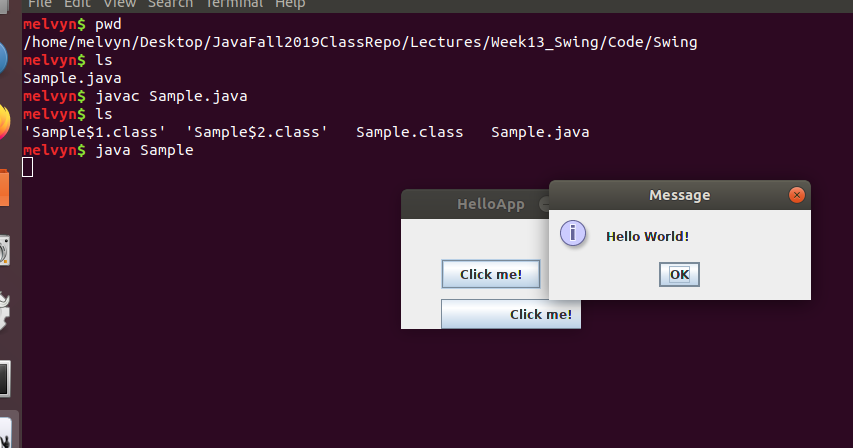
\includegraphics[width=0.9\textwidth]{Images/templateresult.png}
  \caption{What happens when you run the template code.}
  \label{templateresult}
\end{figure}

Below is the source code for the template. As always, the code can be found in
the class repo. The code for this week is in
\textit{Week13\_Swing/Code/Swing/Sample.java}

\lstinputlisting{Code/Swing/Sample.java}

Notice that there are calls to the following functions:
\begin{enumerate}
\item \textit{setBounds()}
\item \textit{setTitle()}
\item \textit{setResizeable()}
\item \textit{addActionListener()}
\item \textit{showMessageDialog()}
\end{enumerate}

Let's take a minute to play with these functions and see what they do ( make
sure to change the showMessageDialog() call in addActionListener(), but don't
acturally change action listener. That can get tricky. )

\subsection{Extra Credit}
See if you can accomplish the task and I'll give you an extra credit! Ready?
Set.... Go!
\end{document}

